The following literature review is to present and clearly define the terms and definitions regarding database technology. The structure of this section begins to define the following principles; ACID compliance and the CAP theorem. The relational model will be explained to elaborate how the classic relational database came to be. The shortfalls of relational databases will then be used to introduce what NoSQL technology is, and how this contrasts with the many variations of NoSQL databases including key-value, column family, and document stores.

A summary will conclude how each section ties into the scope of this project and why research into our problem definition will bring value to spatio-temporal data mining, analysis, and visualization.

\subsection{ACID Compliance}
\label{sec:acid}

From an article written in \emph{Database Guide} \cite{acid}; Atomicity, Consistency, Isolation, Durability (ACID) are the properties that can guarantee that transaction based databases perform reliably. These properties concern themselves over how databases recover after failures such as a transaction, system, or media failure.

\paragraph{Atomicity}
A single transaction could be comprised of one or more steps, and if one of them fails then the transaction will only be partially successful. Atomicity guarantees that if one step fails, the whole transaction fails and the state of the database will be rolled back to a state prior to the transaction.

\paragraph{Consistency}
Data may need to conform to a variety of rules and constraints, especially with regard to relational databases. If any data does not conform to these rules or the set schema, it will not be consistent with the rest of the database. Allowing this data to become a part of the database means that we cannot guarantee our predefined rules. This is one of the properties that NoSQL databases relax on in order to provide higher availability and partition tolerance. A consistent database will ensure that any data being inserted into the database will follow all the predefined rules or else the transaction will be rejected.

\paragraph{Isolation}
To avoid transaction conflicts, each transaction needs to be performed in isolation. This means that no transaction will affect another, and if necessary, will take precedence of one over another in the event of a conflict.

\paragraph{Durability}
For a database to be reliable in the event of any of the aforementioned failures, if a transaction has been committed, it needs to be able to guarantee that the transaction has been stored permanently. Durability along with atomicity work together to keep a database reliable when faced with a failure either during or directly after a transaction as been committed.

A database that is ACID-compliant is robust against data being corrupted during a failure and guarantees that only successful transactions are processed.

\subsection{CAP Theorem}
\label{cap}
Gilbert \& Lynch \cite{cap} explain that, in distributed systems, there is often a trade-off between consistency, availability, and network partition tolerance (CAP). Eric Brewer presented this theorem in the context of geographically separated datacenters supporting web services implicating that a multi-node database cannot ensure all three properties under CAP. Following this web service context, the three properties are described as follows:

\begin{itemize}
    \item \textbf{Consistency} means that the server will return the correct response to each request.
    \item \textbf{Availability} will guarantee that every request will receive a response.
    \item \textbf{Partition tolerance} refers to the system implementation allowing the database to be split into multiple groups unable to communicate with one another.
\end{itemize}

Gilbert \& Lynch, when referring to these properties, say:

\begin{quote}
    ``CAP states that any protocol implementing an atomic read/write register cannot guarantee both safety and liveness in a system prone to partitions.''
\end{quote}

The CAP theorem illustrates the trade-off between safety and liveness when considering an unreliable system. For the safety property to hold, every point in each step of a transaction should be atomically consistent. For the liveness property to hold, a desirable outcome should result as long as the execution continues for long enough.

\subsection{Relational Database}

Edgar F. Codd, an IBM fellow, was responsible for proposing the idea about the relational model \cite{relational-db}. The relational model came as a solution to the problem in the distinction between the logical view and physical representation of the data being stored. This was the main issue with the database management systems of the late sixties. Other issues included having programmers follow large pointer chains to access data and redesign programs whenever storage layout structure had to be reconfigured (such as the introduction of indexing).

The relational model solved these issues by providing a clear boundary between the logical and physical representation of data, create a simple model that could be understood by all programmers, and introduce high level language concepts.

The model's structure stores data in tuples with relations represented as tables. Each tuple has attributes, primary and candidate keys. Each attribute has a domain which is the data type of the attribute's values. The tuples became rows and attributes the columns for each row under their respective tables. Furthermore, the degree refers to the number of columns in a table whereas cardinality the number of rows in a table. An illustration of this can be seen in figures \ref{fig:relational-database} and \ref{fig:foreign-key}.

\begin{figure}[h!]
    \centering
    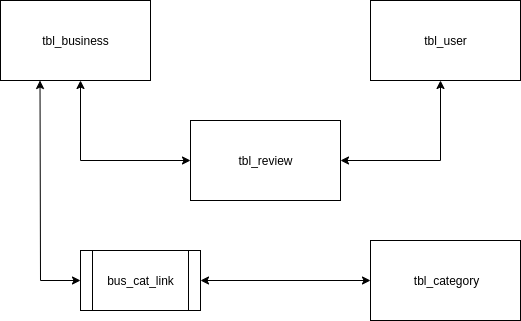
\includegraphics[width=12cm]{img/relational-database.png}
    \caption{A simplified representation of the Yelp dataset in a relational database context illustrating tables and their relations.}
    \label{fig:relational-database}
\end{figure}

\begin{figure}[h!]
    \centering
    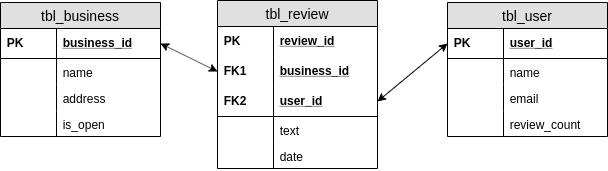
\includegraphics[width=13cm]{img/foreign-key.png}
    \caption{A closeup on the foreign key and primary key structure within the business, user, and review tables.}
    \label{fig:foreign-key}
\end{figure}

The high level language concepts introduced are the algebraic operators we see in SQL today such as \verb|SELECT|, \verb|UNION|, \verb|JOIN|, etc. These operators allow users to convert relations (tables) into other relations (resulting in tables as output).

Since the 1970's, relational database management systems have been the leading database technology with a variety of capabilities and language dialects. This was until NoSQL obtained traction among large Internet corporations and was implemented in the form of distributed, non-relational databases in the 2000s \cite{data-in-nosql}.

\subsection{NoSQL Database}
\label{nosql-database}

NoSQL databases were created to address the shortfalls in classic relational databases when used for data of large volume, variety, and velocity \cite{nosql-db}. Many of these issues were introduced with the increasing popularity of the Internet and systems hosted in the cloud. Relational databases scale poorly over multiple nodes and on large volumes of data which is why SQL databases could no longer be used as the data solution for major Internet companies such as Facebook, Amazon, and Google.

NoSQL database technologies are non-relational and use non-SQL languages to manipulate and query the data. NoSQL is designed to run on multiple nodes (distributed systems), scale horizontally, and some even implementing technologies such as massively parallel processing (MPP) \cite{tigergraph-mpp} or in-memory processing (such as H-store \cite{hstore}). NewSQL is a distributed SQL technology which implements NoSQL features to achieve ACID-compliance (alongside partition tolerance) in any case so they will not be referred to as relational database technology when mentioned in this paper \cite{nosql-db}.

A main challenge for non-relational database systems is the conflict between high availability in distributed systems and remaining transaction based and ACID-complaint (see Subsection \ref{sec:acid}). This results in NoSQL DBMS to typically choose availability and partition tolerance over consistency (see Subsection \ref{cap}) and have become BASE (Basically Available, Soft-state, Eventually consistent)-type systems to compensate \cite{base}. Not all NoSQL databases follow this trend and there are some vendors such as Neo4j and OrientDB that are fully ACID compliant \cite{acid}.

NoSQL databases fall under a broad scope and, in this paper, they will be classified under four categories; key-value stores, document stores, column family (or wide-column) stores, and graph databases.

\paragraph{Key-Value Store}

The basis of a key-value store is that the data is organized in the form of key-value pairs. The key is typically a numeric or string value whereas the value can be any data object or collection of data objects (where a list would be represented by multiple entries of the same key). Each document has a unique identifier with a list of attributes, the key-value paired data. A simple example of this can be seen in Figure \ref{fig:keyvalue}.

\begin{figure}[h!]
    \centering
    \begin{tabular}{ |p{2cm}|p{6cm}|}
        \hline
        \rowcolor{Gray}
        \multicolumn{2}{|c|}{Businesses} \\
        \hline
        \rowcolor{LightGray}
        Key & Attributes                 \\
        \hline
        0   & Name: ``McDonald's''       \\
            & Categories: ``Fast-food''  \\
            & Categories: ``Takeaway''   \\
            & Stars: 2.5                 \\
            & Open: true                 \\
        \hline
        1   & Name: ``KFC''              \\
            & Categories: ``Fast-food''  \\
            & Categories: ``Restaurant'' \\
            & Stars: 3.0                 \\
            & Open: true                 \\
        \hline
    \end{tabular}
    \vspace*{5mm}
    \caption{An example of business entries stored in a key-value store.}
    \label{fig:keyvalue}
\end{figure}

Castellano \cite{keyvalue-article} explains that key-value stores are designed to be lightning fast, simple, and unstructured. They expose three operations namely; \verb|PUT|, \verb|GET|, and \verb|DELETE|, with some implementations adding an additional operation, \verb|SEARCH|, that matches keys or key-value pairs given a specified search expression and key namespace. These databases are decentralized in nature so find difficulty in providing the transactional guarantees of ACID.

\paragraph{Document Store}

As the name suggests, document store databases store their data in the form of documents. Typically, the document formats are JSON, XML, PDF, etc. Unlike key-value stores, document stores are semi-structured and both keys and values are fully searchable \cite{nosql-db}. Document stores are still schema-less and are well suited for data that is dissimilar such as those which do not fit well in a table with set columns \cite{docstore-article} or require many ``nulls''. These databases, like key-value stores, do not perform well if the data is highly relational and requires some kind of normalization.

\paragraph{Column Family Store}

Manoj \cite{docstore-article} explains column families as more structured data stores in that they store data in columns. They are a hybrid row/column store but store their data in distributed architectures instead of tables. Data is stored in a column-family (analogous to a table in SQL) but column-families have no relation to one another unlike in relational models. Column-families are less flexible than the previous key-value and document store databases as one will have to predefine a column family's attributes and are grouped together under keyspaces. A column-family model is illustrated in Figure \ref{fig:colfam}.

\begin{figure}[h!]
    \centering
    \begin{tabular}{ |p{6cm}|p{6cm}|}
        \hline
        \rowcolor{Gray}
        \multicolumn{2}{|c|}{Yelp Keyspace}                      \\
        \hline
        \rowcolor{LightGray}
        Users Column-Family         & Businesses Column-Family   \\
        \hline
        RowID: 0                    & RowID: 0                   \\
        FirstName: ``David''        & Name: ``McDonald's''       \\
        Email: ``david@sun.ac.za''  & Categories: ``Fast-food''  \\
        ReviewCount: 8              & Categories: ``Takeaway''   \\
                                    & Stars: 2.5                 \\
                                    & Open: true                 \\
        \hline
        RowID: 2                    & RowID: 4                   \\
        FirstName: ``Kyle''         & Name: ``KFC''              \\
        Email: ``kyle@hotmail.com'' & Categories: ``Fast-food''  \\
        ReviewCount: 3              & Categories: ``Restaurant'' \\
                                    & Stars: 3.0                 \\
                                    & Open: true                 \\
        \hline
    \end{tabular}
    \vspace*{5mm}
    \caption{An example of user and business column-families.}
    \label{fig:colfam}
\end{figure}

\paragraph{Graph}

Graph databases, the focus of this paper, applies a graph structure to store and manipulate data. Data can be stored as key-pair attributes on both the vertices or edges of the database (as can be seen in Figure \ref{fig:graph-db}). Edges can be unidirectional or bidirectional which may add more information about the kind of relation between two edges. Graph databases are the only NoSQL databases in the four classifications of this section that concern themselves with relations and can be visualized easily in a more human-friendly manner \cite{nosql-db}.

Graph databases are strong at finding patterns and revealing information about the relationship between vertices rather than aggregate queries on the data itself.

Within the category of graph databases we find three main subcategories; property (or attributed) graphs, hypergraphs, and resource description framework (RDF) triples \cite{socialdata}. The type of graph databases focused on in this investigation are property graphs.

\begin{figure}[h!]
    \centering
    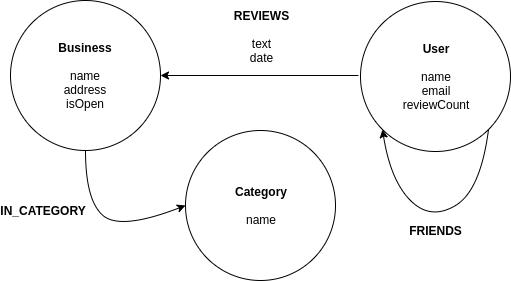
\includegraphics[width=12cm]{img/graph-db.png}
    \caption{A simplified representation of the Yelp dataset in a property graph database context illustrating vertices, edges, and their attribute keys.}
    \label{fig:graph-db}
\end{figure}

\subsection{Summary}

From the literature above, we face the following questions:

\begin{quote}
    \textbf{What would make a non-relational solution more suitable than a relational solution?}
\end{quote}

Moniruzzaman \& Hossain \cite{nosql-db} elaborate the shortcomings of relational database technologies in terms of performance when distributed over geographically diverse datacenters due to their strong emphasis on consistency while maintaining ACID-compliance. As emphasized by Chen \cite{socialdata} \& Makris et. al. \cite{mongovspostgres}, due to the trend of services hosted in the cloud and velocity of incoming data and requests, a horizontally scalable, distributed system would be best suited to address these issues -- which would suggest a NoSQL solution.

\begin{quote}
    \textbf{When compared among other NoSQL databases, what makes a graph database solution stand out?}
\end{quote}

Spatial data is often highly relational due to the ties between vertices representing physical locations and their association with other entities in the database. This means the data will be closely related and that trend will follow in how the queries are written. Chen \cite{socialdata} explains that the queries in a graph database are designed to reveal hidden trends among the relationships in the data (especially when visualized) rather than within the data itself adding additional value in this implementation.

Time adds an ordinal relation among all entries in the data that hold this property. Due to graph databases being the most relational among the NoSQL databases and their ability to ask complex questions to complex data. These complex questions would be multi join-style queries which are typically expensive but due to a graph's relational architecture, graph databases should be more well suited in comparison to other NoSQL database solutions handling this semi-structured data \cite{data-in-nosql}.

\begin{quote}
    \textbf{Why compare a relational solution to a graph database and not another NoSQL solution?}
\end{quote}

Relational databases should come close due to their ability to manipulate data based on table relations. Their lack of scalability may see them lose in terms of overall benchmark performance when tested on large volumes of this kind of data, especially due to how join-style queries scale with table size \cite{data-in-nosql}.

Makris, et. al. \cite{mongovspostgres} compares how MongoDB (with GeoJSON) and PostgreSQL (with PostGIS) perform against one another on spatial data and show that PostgreSQL outperforms its NoSQL rival. Referring to the content in Subsection \ref{nosql-database} it doesn't come as a surprise due to the lack of suitability relational queries are for document store databases. This means that complex queries perform poorly for a database such as MongoDB. One important observation that this paper does point out is how well PostgreSQL performed despite the volume of data. This suggests that the scalability issue was not as prominent as how well these complex queries were handled.

\begin{quote}
    \textbf{Why spatio-temporal data?}
\end{quote}

Spatio-temporal data is constantly being generated by GPS-equipped devices everyday \cite{twitterdata}\cite{clost}. This data has important applications in epidemiologic \cite{spatiotemporal-epidemiology}, marine, disaster relief, and social data investigation \cite{rao2012spatiotemporal}. Few papers address a graph database solution for spatio-temporal data but due to its importance and abundance it would be important to seek an appropriate technology to store, model, and visualize these datasets.

\paragraph{In conclusion} The findings in this paper would answer which technology, graph or relational, would perform the best not only in benchmark performance but suitability in terms of querying, modelling, and visualizing spatio-temporal data. This answer will be useful if one would like to perform analysis on not only a spatio-temporal dataset, but also investigate relations among the data with a suitable database, and perform/write efficient queries.